First, we describe the mult-agent surveillance synthesis problem informally, in the context of a motivating case study. 

We consider wildlife conservation in Africa, in particular, at the Selous Game Reserve (SGR) located in Tanzania, where the African Black Rhinoceros population is under serious threat due to poaching. 

As an answer to a recommended anti-poaching initiative in the SGR by the World Heritage Centre,  we propose using a sensor network for tracking the position of a potential poacher  with user-specified precision. Since the SGR is a very large area, the network consists of both mobile and static sensors. We apply the  distributed synthesis method proposed in this paper to synthesize surveillance strategies for the mobile sensors that satisfy the desired tracking requirement.

%Recommendations of the report include, inter alia, an anti-poaching initiative focused in the SGR. This is a very large environment and so we propose a method using multiple mobile sensors that work with static sensors.  If a surveillance strategy can be synthesized for all the mobile sensors then the location of any potential poachers can be tracked to a user specified requirement. This will allow the authorities to narrow down the position of the target until the situation can be dealt with. 

\begin{figure}
\subfloat[SGR interior landscape \cite{UN13} \label{fig:SGR-map}]{
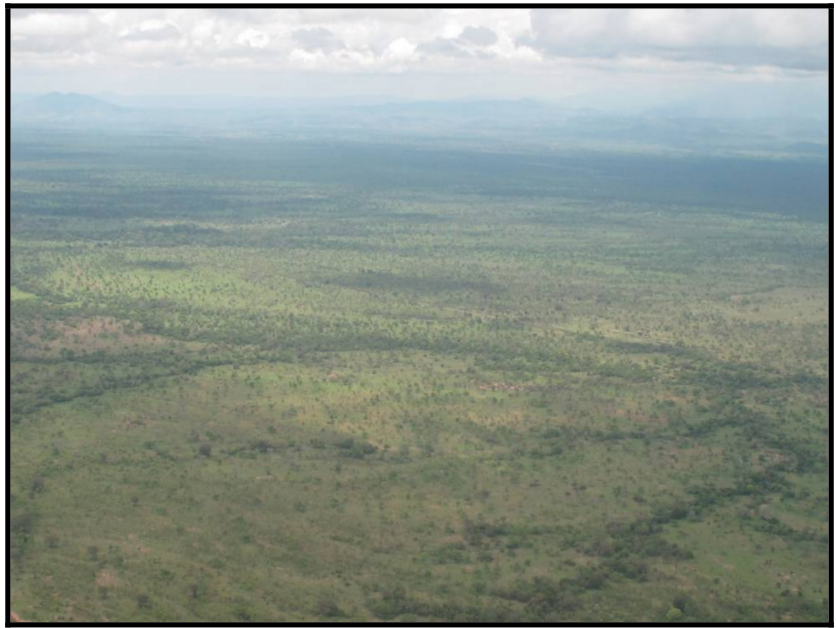
\includegraphics[scale=0.2]{figs/SGR.png}
\hspace{.3cm}}
%\hfill
\subfloat[Gridworld representation of landscape in \ref{fig:SGR-map} \label{fig:SGR-grid}]{
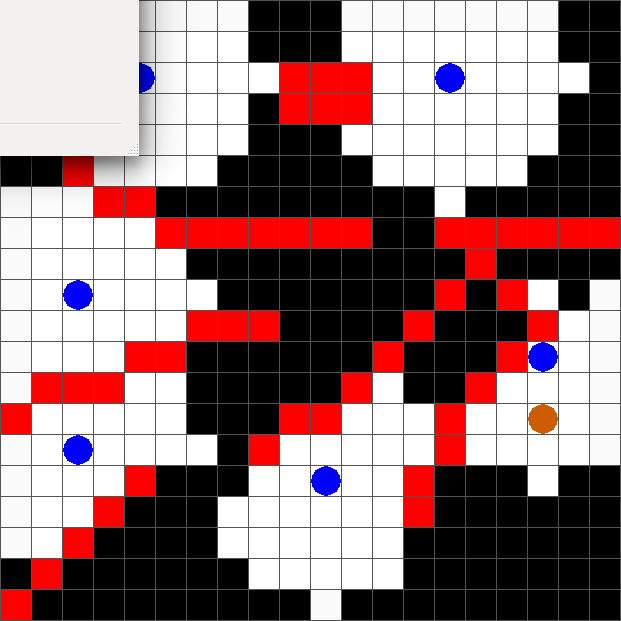
\includegraphics[scale=0.2]{figs/SGR-grid-vis.png}
}


\caption{The landscape in \ref{fig:SGR-map} is coarsely represented as the gridworld in \ref{fig:SGR-grid}. Te red regions represent impassable terrain. The yellow areas covered are by static sensors.}
\label{fig:casestudy}
\end{figure}

Figure \ref{fig:casestudy} shows a section of the SGR that we represent as a gridworld which will form the state space of the game. We model the mobile sensors as having an omnidirectional vision with limited range. Each static sensor monitors a given area of the grid (shown in yellow) and detects any presence of the target (i.e., threat) in these states. It cannot however determine the target's exact location. The tracking requirement is to ensure that over and over again, the set of potential location of the target is reduced to $5$ cells. In other words, every time the target escapes from the vision of all the sensors, the network guarantees that eventually the uncertainty about its position will be reduced to $5$ grid cells.

In the next sections we  define this problem formally.
